%\documentclass[a4paper,fleqn,longmktitle]{cas-dc}
\documentclass[a4paper,fleqn]{cas-dc}

%\usepackage[authoryear,longnamesfirst]{natbib}
%\usepackage[authoryear]{natbib}
\usepackage[numbers]{natbib}

\newcommand{\avail}[2]{\noindent {\bf#1:}~{#2}\newline}


%%%Author definitions
\def\tsc#1{\csdef{#1}{\textsc{\lowercase{#1}}\xspace}}
\tsc{WGM}
\tsc{QE}
\tsc{EP}
\tsc{PMS}
\tsc{BEC}
\tsc{DE}
%%%

\begin{document}
\let\WriteBookmarks\relax
\def\floatpagepagefraction{1}
\def\textpagefraction{.001}
\shorttitle{Watershed Workflow}
\shortauthors{E.T. Coon}

\title [mode = title]{Watershed Workflow: a workflow library for integrated hydrologic models.}                      
\tnotemark[1]

\tnotetext[1]{BLAH BLAH BLAH US Government reserves all writes.}

\author[1]{Ethan T. Coon}[type=editor,
                      auid=000,
                      orcid=0000-0001-8124-9622]
\cormark[1]
\ead{coonet@ornl.gov}
\credit{Conceptualization, Software, Authorship}
\address[1]{Climate Change Science Institute \& Environmental Sciences Division, Oak Ridge National Laboratory, 1 Bethel Valley Road, Oak Ridge, TN, 37830, USA}
\cortext[cor1]{Corresponding author}

\begin{abstract}
Watershed workflow does really cool stuff.
Watershed workflow does really cool stuff.
Watershed workflow does really cool stuff.
Watershed workflow does really cool stuff.
Watershed workflow does really cool stuff.
Watershed workflow does really cool stuff.
\end{abstract}

\begin{graphicalabstract}
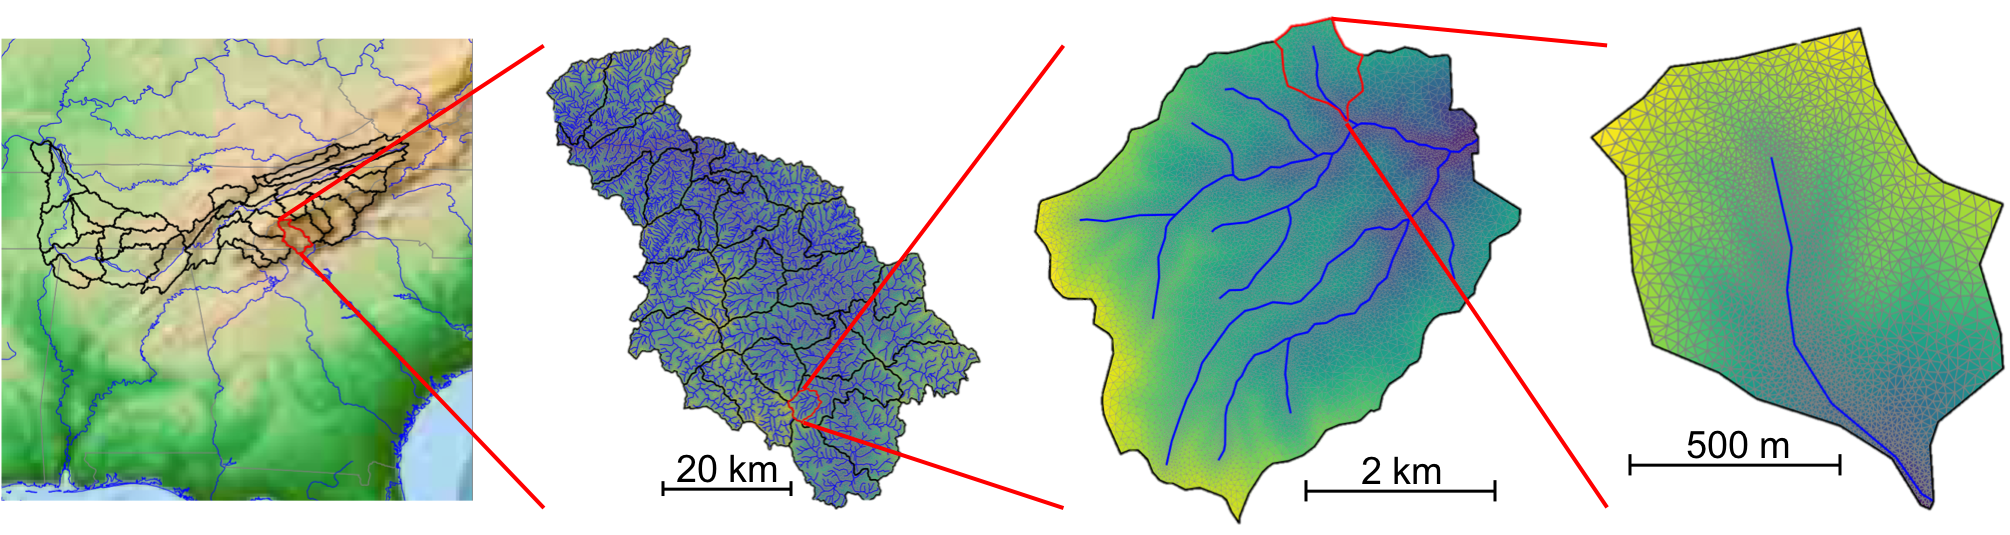
\includegraphics[width=\textwidth]{figs2/watersheds/watershed_workflow.png}
\end{graphicalabstract}

\begin{highlights}
\item Research highlights item 1
\item Research highlights item 2
\item Research highlights item 3
\end{highlights}

\begin{keywords}
integrated hydrologic modeling \sep modeling workflow \sep watershed 
\end{keywords}


\maketitle

\section*{Software availability}
%
\avail{Software name}{Watershed Workflow}
\avail{Developer}{Ethan Coon}
\avail{Year first official release}{2020}
\avail{Hardware requirements}{PC}
\avail{System requirements}{Windows, Linux, Mac}
\avail{Program language}{Python3}
\avail{Program size}{2 MB}
\avail{Availability}{\url{https://github.com/ecoon/watershed-workflow}}
\avail{License}{BSD 3-clause}
\avail{Documentation}{User guide, API documentation, and examples hosted at \url{https://ecoon.github.io/watershed-workflow}}
%
%
\section{Introduction}\label{sec:introduction}
%
\begin{itemize}
\item Integrated hydrology is important
\item Hyper-resolution hydro
\item remote sensing and FAIR data
\item High performance computing
\item Models are powerful but require large setup and difficult learning curve
\item Workflows and software abstractions offer opportunities to provide middleware.
\item Lit review.
\item Watershed Workflow is...
\end{itemize}

\section{A worked example: the Coweeta Hydrologic Laboratory}\label{sec:example}
\begin{itemize}
\item Jupyter notebook
\item Resulting mesh
\item Simulation output
\end{itemize}

\section{Data Sources and Acquisition}\label{sec:acquisition}
%
\begin{itemize}
\item Wide variety of data needs for watershed models.
\item Open data portals and synthesis products provided by government agencies provide broad coverage with discoverable data.
\item ReST APIs make data discoverable.
\end{itemize}

\subsection{Watershed geometry}\label{ssc:acquisition:geom}
%
\begin{itemize}
\item 
\end{itemize}

\subsection{Land Cover}\label{ssc:acquisition:land_cover}
%
Land cover is important for surface and vegetative processes.  
\begin{itemize}
\item Energy balance, controls ET
\item Urban, impervious surfaces
\item Land cover change
\item NLCD dataset
\end{itemize}
  
\subsection{Subsurface structure and soil properties}\label{ssc:acquisition:soil}
%
\begin{itemize}
\item Key sensitive parameter for integrated hydrology is the subsurface structure and soil properties
\item NRCS soils dataset
\item Often more info provided by users -- depth to bedrock map, geologic maps, etc.
\end{itemize}

\subsection{Meteorological data}\label{ssc:acquisition:met}
%
\begin{itemize}
\item Time-dependent data typically should not be projected onto the mesh.
\item Rasters stored as HDF5 data and should be projected onto the mesh by the code.
\item In the future, may support more generic models for both downscaling and upscaling?
\end{itemize}

\subsection{Data discovery and coverage}\label{ssc:acquisition:coverage}
%
\begin{itemize}
\item ReST APIs and open data portals allow automatic dataset discovery.
\item Coverage is all of US for the currently implemented sources.
\end{itemize}

\subsection{User-provided data}\label{ssc:acquisition:user}
%
\begin{itemize}
\item shapefile
\item raster
\end{itemize}


\section{Data Curation}\label{sec:data_curation}
%
\begin{itemize}
\item Coordinate transformation
\item Working across scales: data smoothing, simplification, and coarsening
\item DEM conditioning
\end{itemize}

\section{Mesh Generation}\label{sec:meshes}
%
\begin{itemize}
\item 
\end{itemize}

\section{Software Design}\label{sec:approach}
%
\begin{itemize}
\item Python libraries for code, Jupyter notebooks for orchestration
\item Source abstraction -- shape vs raster
\item Extensible -- not limited to ATS.
\item Open source libraries for GIS (fiona, rasterio, shapely, cartopy, pyproj, QGIS) and geometry (meshpy, triangle).
\item Installation from Anaconda packages
\end{itemize}

\section{Conclusions and Future Work}\label{sec:conclusions}
%
\begin{itemize}
\item 
\end{itemize}


\printcredits

\bibliographystyle{cas-model2-names}
\bibliography{refs}


%\vskip3pt

\bio{figs2/bio/coon.jpg}
Dr. Ethan Coon is a computational hydrologist in the Climate Change Science Institute at ORNL.
He has a background in applied and computational mathematics, and has done research in applying computational methods for the Earth, especially land surface and subsurface processes.
Broadly he is interested in process-based modeling, integrating models with data, and leverage modeling to understand the processes that govern our changing planet.
\endbio


\end{document}

